\documentclass[1p]{elsarticle_modified}
%\bibliographystyle{elsarticle-num}

%\usepackage[colorlinks]{hyperref}
%\usepackage{abbrmath_seonhwa} %\Abb, \Ascr, \Acal ,\Abf, \Afrak
\usepackage{amsfonts}
\usepackage{amssymb}
\usepackage{amsmath}
\usepackage{amsthm}
\usepackage{scalefnt}
\usepackage{amsbsy}
\usepackage{kotex}
\usepackage{caption}
\usepackage{subfig}
\usepackage{color}
\usepackage{graphicx}
\usepackage{xcolor} %% white, black, red, green, blue, cyan, magenta, yellow
\usepackage{float}
\usepackage{setspace}
\usepackage{hyperref}

\usepackage{tikz}
\usetikzlibrary{arrows}

\usepackage{multirow}
\usepackage{array} % fixed length table
\usepackage{hhline}

%%%%%%%%%%%%%%%%%%%%%
\makeatletter
\renewcommand*\env@matrix[1][\arraystretch]{%
	\edef\arraystretch{#1}%
	\hskip -\arraycolsep
	\let\@ifnextchar\new@ifnextchar
	\array{*\c@MaxMatrixCols c}}
\makeatother %https://tex.stackexchange.com/questions/14071/how-can-i-increase-the-line-spacing-in-a-matrix
%%%%%%%%%%%%%%%

\usepackage[normalem]{ulem}

\newcommand{\msout}[1]{\ifmmode\text{\sout{\ensuremath{#1}}}\else\sout{#1}\fi}
%SOURCE: \msout is \stkout macro in https://tex.stackexchange.com/questions/20609/strikeout-in-math-mode

\newcommand{\cancel}[1]{
	\ifmmode
	{\color{red}\msout{#1}}
	\else
	{\color{red}\sout{#1}}
	\fi
}

\newcommand{\add}[1]{
	{\color{blue}\uwave{#1}}
}

\newcommand{\replace}[2]{
	\ifmmode
	{\color{red}\msout{#1}}{\color{blue}\uwave{#2}}
	\else
	{\color{red}\sout{#1}}{\color{blue}\uwave{#2}}
	\fi
}

\newcommand{\Sol}{\mathcal{S}} %segment
\newcommand{\D}{D} %diagram
\newcommand{\A}{\mathcal{A}} %arc


%%%%%%%%%%%%%%%%%%%%%%%%%%%%%5 test

\def\sl{\operatorname{\textup{SL}}(2,\Cbb)}
\def\psl{\operatorname{\textup{PSL}}(2,\Cbb)}
\def\quan{\mkern 1mu \triangleright \mkern 1mu}

\theoremstyle{definition}
\newtheorem{thm}{Theorem}[section]
\newtheorem{prop}[thm]{Proposition}
\newtheorem{lem}[thm]{Lemma}
\newtheorem{ques}[thm]{Question}
\newtheorem{cor}[thm]{Corollary}
\newtheorem{defn}[thm]{Definition}
\newtheorem{exam}[thm]{Example}
\newtheorem{rmk}[thm]{Remark}
\newtheorem{alg}[thm]{Algorithm}

\newcommand{\I}{\sqrt{-1}}
\begin{document}

%\begin{frontmatter}
%
%\title{Boundary parabolic representations of knots up to 8 crossings}
%
%%% Group authors per affiliation:
%\author{Yunhi Cho} 
%\address{Department of Mathematics, University of Seoul, Seoul, Korea}
%\ead{yhcho@uos.ac.kr}
%
%
%\author{Seonhwa Kim} %\fnref{s_kim}}
%\address{Center for Geometry and Physics, Institute for Basic Science, Pohang, 37673, Korea}
%\ead{ryeona17@ibs.re.kr}
%
%\author{Hyuk Kim}
%\address{Department of Mathematical Sciences, Seoul National University, Seoul 08826, Korea}
%\ead{hyukkim@snu.ac.kr}
%
%\author{Seokbeom Yoon}
%\address{Department of Mathematical Sciences, Seoul National University, Seoul, 08826,  Korea}
%\ead{sbyoon15@snu.ac.kr}
%
%\begin{abstract}
%We find all boundary parabolic representation of knots up to 8 crossings.
%
%\end{abstract}
%\begin{keyword}
%    \MSC[2010] 57M25 
%\end{keyword}
%
%\end{frontmatter}

%\linenumbers
%\tableofcontents
%
\newcommand\colored[1]{\textcolor{white}{\rule[-0.35ex]{0.8em}{1.4ex}}\kern-0.8em\color{red} #1}%
%\newcommand\colored[1]{\textcolor{white}{ #1}\kern-2.17ex	\textcolor{white}{ #1}\kern-1.81ex	\textcolor{white}{ #1}\kern-2.15ex\color{red}#1	}

{\Large $\underline{12n_{0426}~(K12n_{0426})}$}

\setlength{\tabcolsep}{10pt}
\renewcommand{\arraystretch}{1.6}
\vspace{1cm}\begin{tabular}{m{100pt}>{\centering\arraybackslash}m{274pt}}
\multirow{5}{120pt}{
	\centering
	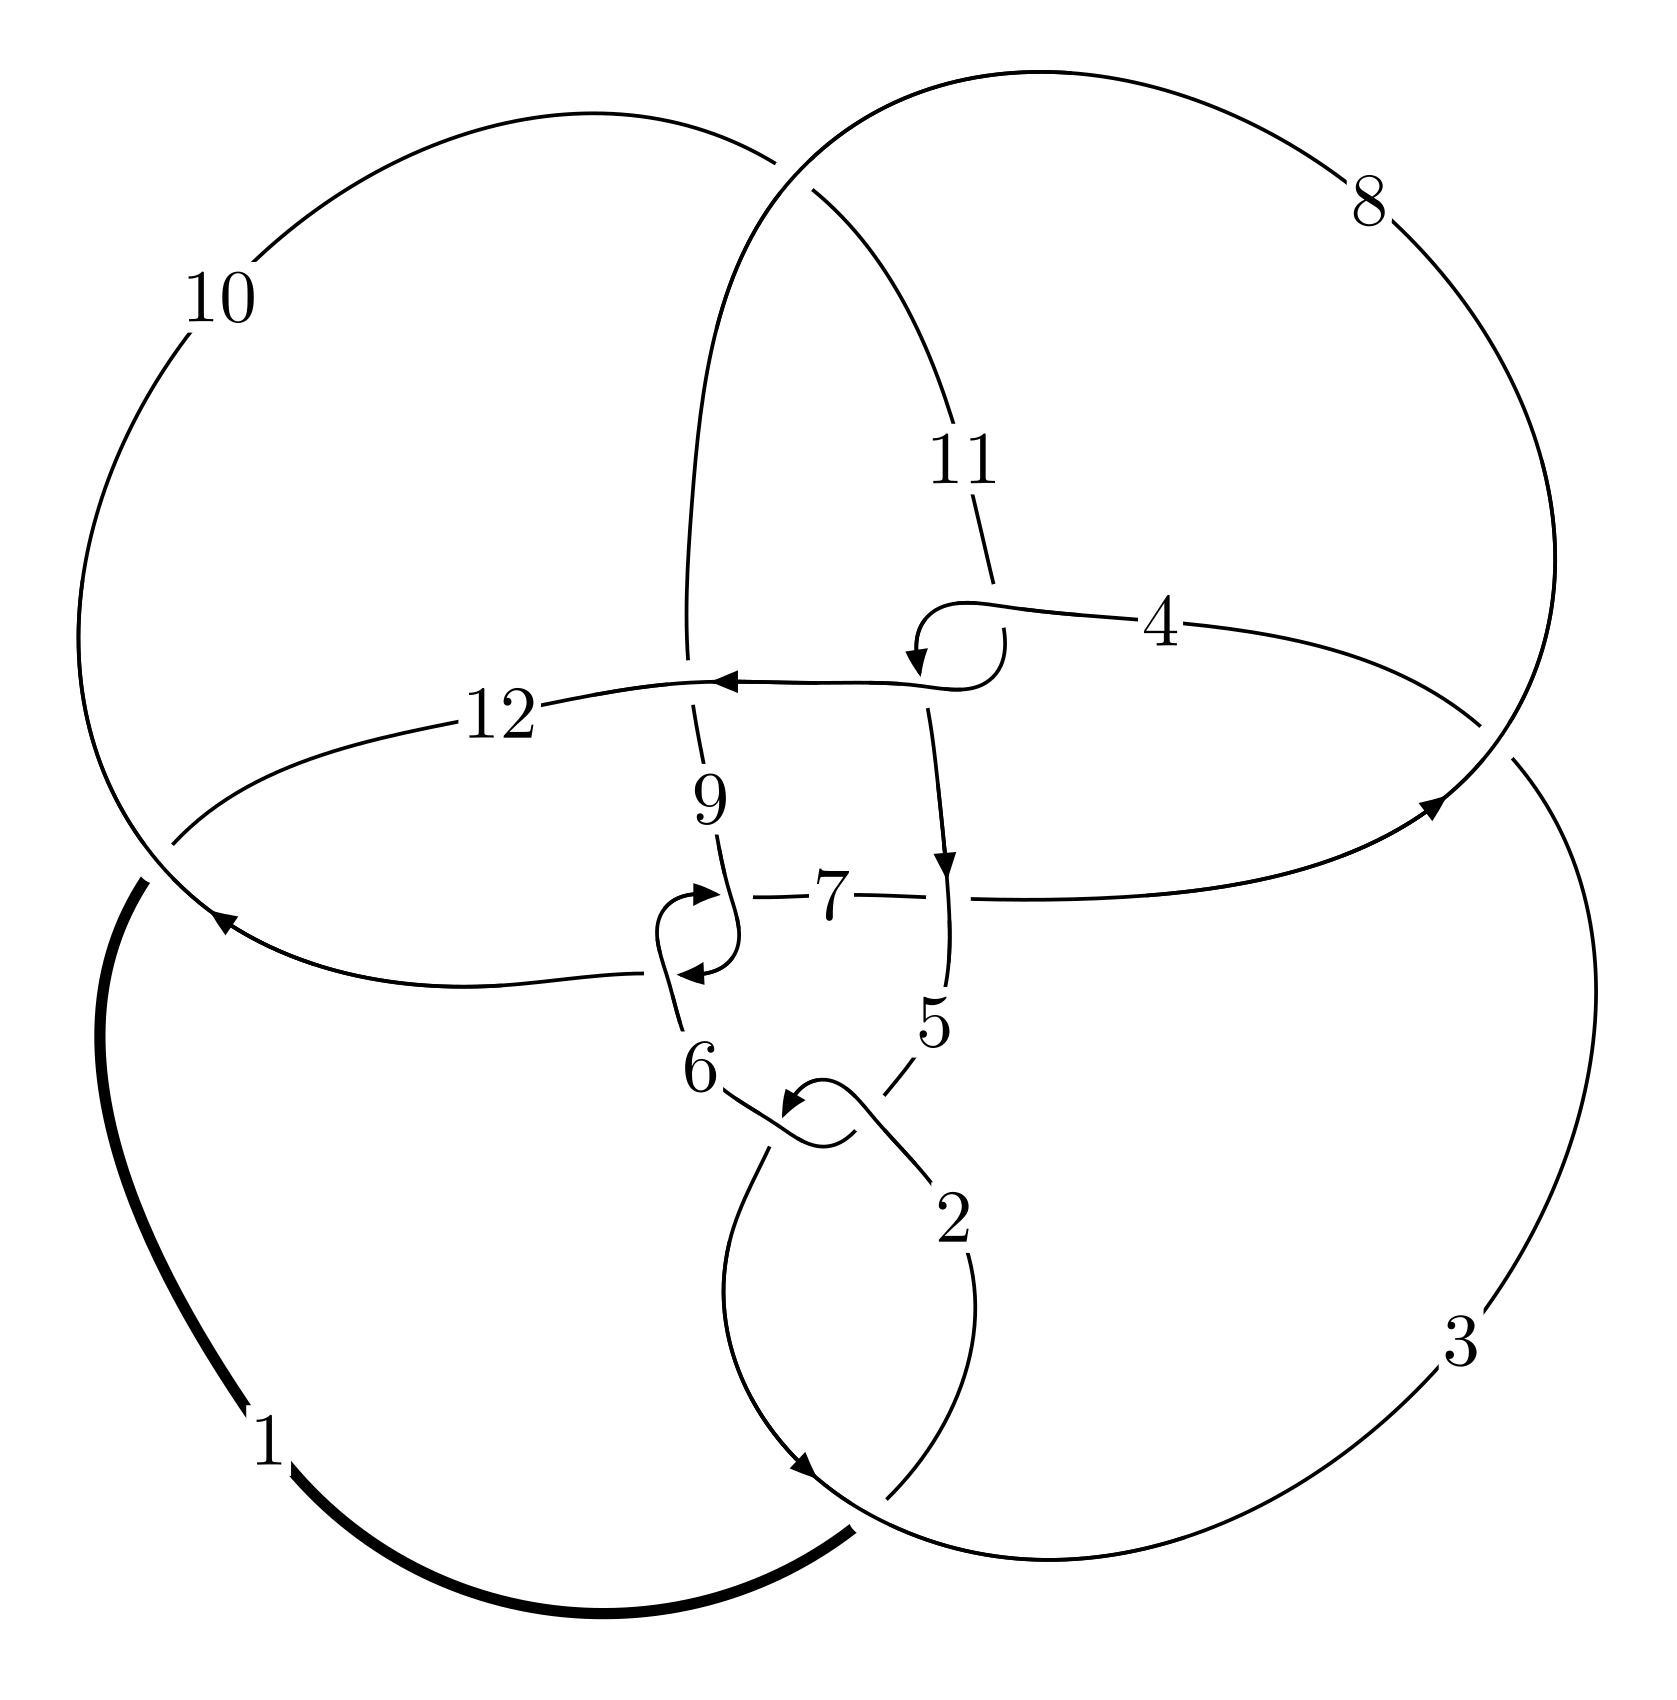
\includegraphics[width=112pt]{../../../GIT/diagram.site/Diagrams/png/2515_12n_0426.png}\\
\ \ \ A knot diagram\footnotemark}&
\allowdisplaybreaks
\textbf{Linearized knot diagam} \\
\cline{2-2}
 &
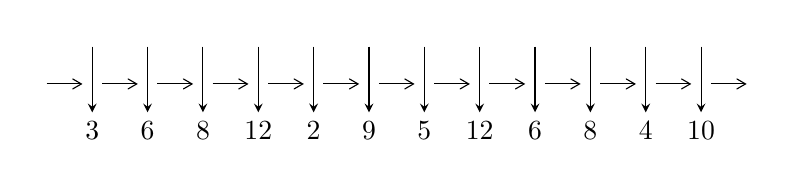
\begin{tikzpicture}[x=20pt, y=17pt]
	% nodes
	\node (C0) at (0, 0) {};
	\node (C1) at (1, 0) {};
	\node (C1U) at (1, +1) {};
	\node (C1D) at (1, -1) {3};

	\node (C2) at (2, 0) {};
	\node (C2U) at (2, +1) {};
	\node (C2D) at (2, -1) {6};

	\node (C3) at (3, 0) {};
	\node (C3U) at (3, +1) {};
	\node (C3D) at (3, -1) {8};

	\node (C4) at (4, 0) {};
	\node (C4U) at (4, +1) {};
	\node (C4D) at (4, -1) {12};

	\node (C5) at (5, 0) {};
	\node (C5U) at (5, +1) {};
	\node (C5D) at (5, -1) {2};

	\node (C6) at (6, 0) {};
	\node (C6U) at (6, +1) {};
	\node (C6D) at (6, -1) {9};

	\node (C7) at (7, 0) {};
	\node (C7U) at (7, +1) {};
	\node (C7D) at (7, -1) {5};

	\node (C8) at (8, 0) {};
	\node (C8U) at (8, +1) {};
	\node (C8D) at (8, -1) {12};

	\node (C9) at (9, 0) {};
	\node (C9U) at (9, +1) {};
	\node (C9D) at (9, -1) {6};

	\node (C10) at (10, 0) {};
	\node (C10U) at (10, +1) {};
	\node (C10D) at (10, -1) {8};

	\node (C11) at (11, 0) {};
	\node (C11U) at (11, +1) {};
	\node (C11D) at (11, -1) {4};

	\node (C12) at (12, 0) {};
	\node (C12U) at (12, +1) {};
	\node (C12D) at (12, -1) {10};
	\node (C13) at (13, 0) {};

	% arrows
	\draw[->,>={angle 60}]
	(C0) edge (C1) (C1) edge (C2) (C2) edge (C3) (C3) edge (C4) (C4) edge (C5) (C5) edge (C6) (C6) edge (C7) (C7) edge (C8) (C8) edge (C9) (C9) edge (C10) (C10) edge (C11) (C11) edge (C12) (C12) edge (C13) ;	\draw[->,>=stealth]
	(C1U) edge (C1D) (C2U) edge (C2D) (C3U) edge (C3D) (C4U) edge (C4D) (C5U) edge (C5D) (C6U) edge (C6D) (C7U) edge (C7D) (C8U) edge (C8D) (C9U) edge (C9D) (C10U) edge (C10D) (C11U) edge (C11D) (C12U) edge (C12D) ;
	\end{tikzpicture} \\
\hhline{~~} \\& 
\textbf{Solving Sequence} \\ \cline{2-2} 
 &
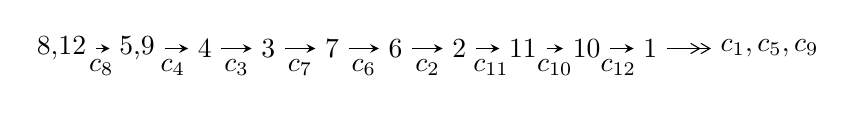
\begin{tikzpicture}[x=23pt, y=7pt]
	% node
	\node (A0) at (-1/8, 0) {8,12};
	\node (A1) at (17/16, 0) {5,9};
	\node (A2) at (17/8, 0) {4};
	\node (A3) at (25/8, 0) {3};
	\node (A4) at (33/8, 0) {7};
	\node (A5) at (41/8, 0) {6};
	\node (A6) at (49/8, 0) {2};
	\node (A7) at (57/8, 0) {11};
	\node (A8) at (65/8, 0) {10};
	\node (A9) at (73/8, 0) {1};
	\node (C1) at (1/2, -1) {$c_{8}$};
	\node (C2) at (13/8, -1) {$c_{4}$};
	\node (C3) at (21/8, -1) {$c_{3}$};
	\node (C4) at (29/8, -1) {$c_{7}$};
	\node (C5) at (37/8, -1) {$c_{6}$};
	\node (C6) at (45/8, -1) {$c_{2}$};
	\node (C7) at (53/8, -1) {$c_{11}$};
	\node (C8) at (61/8, -1) {$c_{10}$};
	\node (C9) at (69/8, -1) {$c_{12}$};
	\node (A10) at (11, 0) {$c_{1},c_{5},c_{9}$};

	% edge
	\draw[->,>=stealth]	
	(A0) edge (A1) (A1) edge (A2) (A2) edge (A3) (A3) edge (A4) (A4) edge (A5) (A5) edge (A6) (A6) edge (A7) (A7) edge (A8) (A8) edge (A9) ;
	\draw[->>,>={angle 60}]	
	(A9) edge (A10);
\end{tikzpicture} \\ 

\end{tabular} \\

\footnotetext{
The image of knot diagram is generated by the software ``\textbf{Draw programme}" developed by Andrew Bartholomew(\url{http://www.layer8.co.uk/maths/draw/index.htm\#Running-draw}), where we modified some parts for our purpose(\url{https://github.com/CATsTAILs/LinksPainter}).
}\phantom \\ \newline 
\centering \textbf{Ideals for irreducible components\footnotemark of $X_{\text{par}}$} 
 
\begin{align*}
I^u_{1}&=\langle 
- u^6+2 u^5- u^4- u^3- u^2+3 b+u-1,\;5 u^6-16 u^5+11 u^4+20 u^3-19 u^2+6 a-14 u+14,\\
\phantom{I^u_{1}}&\phantom{= \langle  }u^7-4 u^6+5 u^5+2 u^4-7 u^3+6 u-2\rangle \\
I^u_{2}&=\langle 
- u^5-2 u^4+u^3+3 u^2+b+u-1,\;3 u^5+4 u^4-10 u^3-11 u^2+2 a+5 u+12,\\
\phantom{I^u_{2}}&\phantom{= \langle  }u^6+2 u^5-2 u^4-5 u^3- u^2+4 u+2\rangle \\
I^u_{3}&=\langle 
b+u,\;a+u,\;u^2+u-1\rangle \\
I^u_{4}&=\langle 
b- a- u-1,\;a^2+a u+2 a+2 u+1,\;u^2+u-1\rangle \\
I^u_{5}&=\langle 
u^3-2 u^2+b+2 u-1,\;- u^3+2 u^2+a-3 u+2,\;u^4-2 u^3+4 u^2-3 u+1\rangle \\
\\
\end{align*}
\raggedright * 5 irreducible components of $\dim_{\mathbb{C}}=0$, with total 23 representations.\\
\footnotetext{All coefficients of polynomials are rational numbers. But the coefficients are sometimes approximated in decimal forms when there is not enough margin.}
\newpage
\renewcommand{\arraystretch}{1}
\centering \section*{I. $I^u_{1}= \langle - u^6+2 u^5- u^4- u^3- u^2+3 b+u-1,\;5 u^6-16 u^5+\cdots+6 a+14,\;u^7-4 u^6+5 u^5+2 u^4-7 u^3+6 u-2 \rangle$}
\flushleft \textbf{(i) Arc colorings}\\
\begin{tabular}{m{7pt} m{180pt} m{7pt} m{180pt} }
\flushright $a_{8}=$&$\begin{pmatrix}1\\0\end{pmatrix}$ \\
\flushright $a_{12}=$&$\begin{pmatrix}0\\u\end{pmatrix}$ \\
\flushright $a_{5}=$&$\begin{pmatrix}-\frac{5}{6} u^6+\frac{8}{3} u^5+\cdots+\frac{7}{3} u-\frac{7}{3}\\\frac{1}{3} u^6-\frac{2}{3} u^5+\cdots-\frac{1}{3} u+\frac{1}{3}\end{pmatrix}$ \\
\flushright $a_{9}=$&$\begin{pmatrix}1\\u^2\end{pmatrix}$ \\
\flushright $a_{4}=$&$\begin{pmatrix}-\frac{5}{6} u^6+\frac{8}{3} u^5+\cdots+\frac{7}{3} u-\frac{7}{3}\\\frac{2}{3} u^6-\frac{7}{3} u^5+\cdots-\frac{8}{3} u+\frac{5}{3}\end{pmatrix}$ \\
\flushright $a_{3}=$&$\begin{pmatrix}-\frac{1}{6} u^6+\frac{1}{3} u^5+\cdots-\frac{1}{3} u-\frac{2}{3}\\\frac{2}{3} u^6-\frac{7}{3} u^5+\cdots-\frac{8}{3} u+\frac{5}{3}\end{pmatrix}$ \\
\flushright $a_{7}=$&$\begin{pmatrix}\frac{1}{6} u^6-\frac{1}{3} u^5+\cdots-\frac{2}{3} u+\frac{5}{3}\\\frac{1}{3} u^6-\frac{2}{3} u^5+\cdots-\frac{4}{3} u+\frac{1}{3}\end{pmatrix}$ \\
\flushright $a_{6}=$&$\begin{pmatrix}-\frac{1}{6} u^6+\frac{1}{3} u^5+\cdots-\frac{1}{3} u+\frac{4}{3}\\- u^6+3 u^5-2 u^4-3 u^3+2 u^2+2 u-1\end{pmatrix}$ \\
\flushright $a_{2}=$&$\begin{pmatrix}-\frac{1}{2} u^6+u^5+\frac{1}{2} u^4-3 u^3+\frac{1}{2} u^2+2 u-1\\-\frac{1}{3} u^6+\frac{2}{3} u^5+\cdots+\frac{7}{3} u-\frac{1}{3}\end{pmatrix}$ \\
\flushright $a_{11}=$&$\begin{pmatrix}-\frac{1}{6} u^6+\frac{1}{3} u^5+\cdots+\frac{2}{3} u+\frac{1}{3}\\\frac{1}{3} u^6-\frac{2}{3} u^5+\cdots-\frac{1}{3} u+\frac{1}{3}\end{pmatrix}$ \\
\flushright $a_{10}=$&$\begin{pmatrix}\frac{1}{6} u^6-\frac{1}{3} u^5+\cdots+\frac{1}{3} u+\frac{2}{3}\\\frac{1}{3} u^6-\frac{2}{3} u^5+\cdots-\frac{1}{3} u+\frac{1}{3}\end{pmatrix}$ \\
\flushright $a_{1}=$&$\begin{pmatrix}\frac{1}{6} u^6-\frac{1}{3} u^5+\cdots+\frac{1}{3} u-\frac{1}{3}\\u^5- u^4-2 u^3+2 u^2+3 u-1\end{pmatrix}$\\&\end{tabular}
\flushleft \textbf{(ii) Obstruction class $= -1$}\\~\\
\flushleft \textbf{(iii) Cusp Shapes $= 2 u^6-6 u^5+4 u^4+6 u^3-10 u-10$}\\~\\
\newpage\renewcommand{\arraystretch}{1}
\flushleft \textbf{(iv) u-Polynomials at the component}\newline \\
\begin{tabular}{m{50pt}|m{274pt}}
Crossings & \hspace{64pt}u-Polynomials at each crossing \\
\hline $$\begin{aligned}c_{1}\end{aligned}$$&$\begin{aligned}
&u^7+6 u^6+27 u^5+62 u^4+93 u^3+76 u^2+36 u+4
\end{aligned}$\\
\hline $$\begin{aligned}c_{2},c_{5},c_{8}\end{aligned}$$&$\begin{aligned}
&u^7+4 u^6+5 u^5-2 u^4-7 u^3+6 u+2
\end{aligned}$\\
\hline $$\begin{aligned}c_{3},c_{4},c_{11}\end{aligned}$$&$\begin{aligned}
&u^7+3 u^6-2 u^5-8 u^4+2 u^3+4 u^2+3 u+1
\end{aligned}$\\
\hline $$\begin{aligned}c_{6},c_{7},c_{9}\\c_{12}\end{aligned}$$&$\begin{aligned}
&u^7- u^6+6 u^5+6 u^4+12 u^3+8 u^2+5 u+1
\end{aligned}$\\
\hline $$\begin{aligned}c_{10}\end{aligned}$$&$\begin{aligned}
&u^7-9 u^6+29 u^5-47 u^4+60 u^3-40 u^2+12 u+4
\end{aligned}$\\
\hline
\end{tabular}\\~\\
\newpage\renewcommand{\arraystretch}{1}
\flushleft \textbf{(v) Riley Polynomials at the component}\newline \\
\begin{tabular}{m{50pt}|m{274pt}}
Crossings & \hspace{64pt}Riley Polynomials at each crossing \\
\hline $$\begin{aligned}c_{1}\end{aligned}$$&$\begin{aligned}
&y^7+18 y^6+171 y^5+338 y^4+1121 y^3+424 y^2+688 y-16
\end{aligned}$\\
\hline $$\begin{aligned}c_{2},c_{5},c_{8}\end{aligned}$$&$\begin{aligned}
&y^7-6 y^6+27 y^5-62 y^4+93 y^3-76 y^2+36 y-4
\end{aligned}$\\
\hline $$\begin{aligned}c_{3},c_{4},c_{11}\end{aligned}$$&$\begin{aligned}
&y^7-13 y^6+56 y^5-90 y^4+50 y^3+12 y^2+y-1
\end{aligned}$\\
\hline $$\begin{aligned}c_{6},c_{7},c_{9}\\c_{12}\end{aligned}$$&$\begin{aligned}
&y^7+11 y^6+72 y^5+134 y^4+110 y^3+44 y^2+9 y-1
\end{aligned}$\\
\hline $$\begin{aligned}c_{10}\end{aligned}$$&$\begin{aligned}
&y^7-23 y^6+115 y^5+575 y^4+608 y^3+216 y^2+464 y-16
\end{aligned}$\\
\hline
\end{tabular}\\~\\
\newpage\flushleft \textbf{(vi) Complex Volumes and Cusp Shapes}
$$\begin{array}{c|c|c}  
\text{Solutions to }I^u_{1}& \I (\text{vol} + \sqrt{-1}CS) & \text{Cusp shape}\\
 \hline 
\begin{aligned}
u &= -0.877051 + 0.401438 I \\
a &= \phantom{-}0.390423 - 0.367676 I \\
b &= \phantom{-}0.173321 - 0.977693 I\end{aligned}
 & \phantom{-}1.59409 + 3.78166 I & -7.32325 - 7.33619 I \\ \hline\begin{aligned}
u &= -0.877051 - 0.401438 I \\
a &= \phantom{-}0.390423 + 0.367676 I \\
b &= \phantom{-}0.173321 + 0.977693 I\end{aligned}
 & \phantom{-}1.59409 - 3.78166 I & -7.32325 + 7.33619 I \\ \hline\begin{aligned}
u &= \phantom{-}1.140270 + 0.557068 I \\
a &= \phantom{-}0.742429 - 0.652700 I \\
b &= \phantom{-}0.353960 + 0.627763 I\end{aligned}
 & -2.78671 - 4.23450 I & -16.3139 + 4.7703 I \\ \hline\begin{aligned}
u &= \phantom{-}1.140270 - 0.557068 I \\
a &= \phantom{-}0.742429 + 0.652700 I \\
b &= \phantom{-}0.353960 - 0.627763 I\end{aligned}
 & -2.78671 + 4.23450 I & -16.3139 - 4.7703 I \\ \hline\begin{aligned}
u &= \phantom{-}0.389062\phantom{ +0.000000I} \\
a &= -1.16362\phantom{ +0.000000I} \\
b &= \phantom{-}0.276584\phantom{ +0.000000I}\end{aligned}
 & -0.727542\phantom{ +0.000000I} & -13.4920\phantom{ +0.000000I} \\ \hline\begin{aligned}
u &= \phantom{-}1.54225 + 1.02576 I \\
a &= -1.051040 + 0.651247 I \\
b &= -1.16557 - 2.38792 I\end{aligned}
 & \phantom{-}4.02380 - 9.18258 I & -12.61674 + 3.92434 I \\ \hline\begin{aligned}
u &= \phantom{-}1.54225 - 1.02576 I \\
a &= -1.051040 - 0.651247 I \\
b &= -1.16557 + 2.38792 I\end{aligned}
 & \phantom{-}4.02380 + 9.18258 I & -12.61674 - 3.92434 I\\
 \hline 
 \end{array}$$\newpage\newpage\renewcommand{\arraystretch}{1}
\centering \section*{II. $I^u_{2}= \langle - u^5-2 u^4+u^3+3 u^2+b+u-1,\;3 u^5+4 u^4-10 u^3-11 u^2+2 a+5 u+12,\;u^6+2 u^5-2 u^4-5 u^3- u^2+4 u+2 \rangle$}
\flushleft \textbf{(i) Arc colorings}\\
\begin{tabular}{m{7pt} m{180pt} m{7pt} m{180pt} }
\flushright $a_{8}=$&$\begin{pmatrix}1\\0\end{pmatrix}$ \\
\flushright $a_{12}=$&$\begin{pmatrix}0\\u\end{pmatrix}$ \\
\flushright $a_{5}=$&$\begin{pmatrix}-\frac{3}{2} u^5-2 u^4+5 u^3+\frac{11}{2} u^2-\frac{5}{2} u-6\\u^5+2 u^4- u^3-3 u^2- u+1\end{pmatrix}$ \\
\flushright $a_{9}=$&$\begin{pmatrix}1\\u^2\end{pmatrix}$ \\
\flushright $a_{4}=$&$\begin{pmatrix}-\frac{3}{2} u^5-2 u^4+5 u^3+\frac{11}{2} u^2-\frac{5}{2} u-6\\u^5+2 u^4-2 u^3-4 u^2+3\end{pmatrix}$ \\
\flushright $a_{3}=$&$\begin{pmatrix}-\frac{1}{2} u^5+3 u^3+\frac{3}{2} u^2-\frac{5}{2} u-3\\u^5+2 u^4-2 u^3-4 u^2+3\end{pmatrix}$ \\
\flushright $a_{7}=$&$\begin{pmatrix}\frac{3}{2} u^5+2 u^4-4 u^3-\frac{9}{2} u^2+\frac{3}{2} u+6\\u^3+u^2-1\end{pmatrix}$ \\
\flushright $a_{6}=$&$\begin{pmatrix}\frac{1}{2} u^5+u^4- u^3-\frac{5}{2} u^2+\frac{1}{2} u+3\\- u^5- u^4+4 u^3+3 u^2-2 u-3\end{pmatrix}$ \\
\flushright $a_{2}=$&$\begin{pmatrix}\frac{3}{2} u^5+2 u^4-4 u^3-\frac{7}{2} u^2+\frac{3}{2} u+4\\u^2+u-1\end{pmatrix}$ \\
\flushright $a_{11}=$&$\begin{pmatrix}-\frac{7}{2} u^5-5 u^4+10 u^3+\frac{23}{2} u^2-\frac{7}{2} u-12\\2 u^5+3 u^4-6 u^3-7 u^2+3 u+7\end{pmatrix}$ \\
\flushright $a_{10}=$&$\begin{pmatrix}-\frac{3}{2} u^5-2 u^4+4 u^3+\frac{9}{2} u^2-\frac{1}{2} u-5\\2 u^5+3 u^4-6 u^3-7 u^2+3 u+7\end{pmatrix}$ \\
\flushright $a_{1}=$&$\begin{pmatrix}\frac{9}{2} u^5+6 u^4-13 u^3-\frac{27}{2} u^2+\frac{9}{2} u+14\\-4 u^5-6 u^4+11 u^3+15 u^2-3 u-15\end{pmatrix}$\\&\end{tabular}
\flushleft \textbf{(ii) Obstruction class $= 1$}\\~\\
\flushleft \textbf{(iii) Cusp Shapes $= - u^4-2 u^3+u^2+2 u-10$}\\~\\
\newpage\renewcommand{\arraystretch}{1}
\flushleft \textbf{(iv) u-Polynomials at the component}\newline \\
\begin{tabular}{m{50pt}|m{274pt}}
Crossings & \hspace{64pt}u-Polynomials at each crossing \\
\hline $$\begin{aligned}c_{1}\end{aligned}$$&$\begin{aligned}
&u^6-8 u^5+22 u^4-33 u^3+33 u^2-20 u+4
\end{aligned}$\\
\hline $$\begin{aligned}c_{2},c_{8}\end{aligned}$$&$\begin{aligned}
&u^6+2 u^5-2 u^4-5 u^3- u^2+4 u+2
\end{aligned}$\\
\hline $$\begin{aligned}c_{3},c_{11}\end{aligned}$$&$\begin{aligned}
&(u^3+2 u^2+1)^2
\end{aligned}$\\
\hline $$\begin{aligned}c_{4}\end{aligned}$$&$\begin{aligned}
&(u^3-2 u^2-1)^2
\end{aligned}$\\
\hline $$\begin{aligned}c_{5}\end{aligned}$$&$\begin{aligned}
&u^6-2 u^5-2 u^4+5 u^3- u^2-4 u+2
\end{aligned}$\\
\hline $$\begin{aligned}c_{6}\end{aligned}$$&$\begin{aligned}
&u^6-3 u^5+3 u^4-3 u^3-3 u^2+4 u-1
\end{aligned}$\\
\hline $$\begin{aligned}c_{7},c_{9},c_{12}\end{aligned}$$&$\begin{aligned}
&u^6+3 u^5+3 u^4+3 u^3-3 u^2-4 u-1
\end{aligned}$\\
\hline $$\begin{aligned}c_{10}\end{aligned}$$&$\begin{aligned}
&u^6+6 u^5+3 u^4-21 u^3-5 u^2+25 u+13
\end{aligned}$\\
\hline
\end{tabular}\\~\\
\newpage\renewcommand{\arraystretch}{1}
\flushleft \textbf{(v) Riley Polynomials at the component}\newline \\
\begin{tabular}{m{50pt}|m{274pt}}
Crossings & \hspace{64pt}Riley Polynomials at each crossing \\
\hline $$\begin{aligned}c_{1}\end{aligned}$$&$\begin{aligned}
&y^6-20 y^5+22 y^4+51 y^3-55 y^2-136 y+16
\end{aligned}$\\
\hline $$\begin{aligned}c_{2},c_{5},c_{8}\end{aligned}$$&$\begin{aligned}
&y^6-8 y^5+22 y^4-33 y^3+33 y^2-20 y+4
\end{aligned}$\\
\hline $$\begin{aligned}c_{3},c_{4},c_{11}\end{aligned}$$&$\begin{aligned}
&(y^3-4 y^2-4 y-1)^2
\end{aligned}$\\
\hline $$\begin{aligned}c_{6},c_{7},c_{9}\\c_{12}\end{aligned}$$&$\begin{aligned}
&y^6-3 y^5-15 y^4-5 y^3+27 y^2-10 y+1
\end{aligned}$\\
\hline $$\begin{aligned}c_{10}\end{aligned}$$&$\begin{aligned}
&y^6-30 y^5+251 y^4-745 y^3+1153 y^2-755 y+169
\end{aligned}$\\
\hline
\end{tabular}\\~\\
\newpage\flushleft \textbf{(vi) Complex Volumes and Cusp Shapes}
$$\begin{array}{c|c|c}  
\text{Solutions to }I^u_{2}& \I (\text{vol} + \sqrt{-1}CS) & \text{Cusp shape}\\
 \hline 
\begin{aligned}
u &= -0.853859 + 0.662904 I \\
a &= \phantom{-}0.452623 - 0.427953 I \\
b &= -0.456155 + 0.029114 I\end{aligned}
 & \phantom{-}1.03690 + 2.56897 I & -11.22670 - 1.46771 I \\ \hline\begin{aligned}
u &= -0.853859 - 0.662904 I \\
a &= \phantom{-}0.452623 + 0.427953 I \\
b &= -0.456155 - 0.029114 I\end{aligned}
 & \phantom{-}1.03690 - 2.56897 I & -11.22670 + 1.46771 I \\ \hline\begin{aligned}
u &= \phantom{-}1.183340 + 0.139351 I \\
a &= -0.020355 + 0.564750 I \\
b &= -0.31715 + 1.43860 I\end{aligned}
 & \phantom{-}1.03690 + 2.56897 I & -11.22670 - 1.46771 I \\ \hline\begin{aligned}
u &= \phantom{-}1.183340 - 0.139351 I \\
a &= -0.020355 - 0.564750 I \\
b &= -0.31715 - 1.43860 I\end{aligned}
 & \phantom{-}1.03690 - 2.56897 I & -11.22670 + 1.46771 I \\ \hline\begin{aligned}
u &= -0.579846\phantom{ +0.000000I} \\
a &= -3.80372\phantom{ +0.000000I} \\
b &= \phantom{-}0.926680\phantom{ +0.000000I}\end{aligned}
 & -13.5883\phantom{ +0.000000I} & -10.5470\phantom{ +0.000000I} \\ \hline\begin{aligned}
u &= -2.07912\phantom{ +0.000000I} \\
a &= -1.06082\phantom{ +0.000000I} \\
b &= -2.38008\phantom{ +0.000000I}\end{aligned}
 & -13.5883\phantom{ +0.000000I} & -10.5470\phantom{ +0.000000I}\\
 \hline 
 \end{array}$$\newpage\newpage\renewcommand{\arraystretch}{1}
\centering \section*{III. $I^u_{3}= \langle b+u,\;a+u,\;u^2+u-1 \rangle$}
\flushleft \textbf{(i) Arc colorings}\\
\begin{tabular}{m{7pt} m{180pt} m{7pt} m{180pt} }
\flushright $a_{8}=$&$\begin{pmatrix}1\\0\end{pmatrix}$ \\
\flushright $a_{12}=$&$\begin{pmatrix}0\\u\end{pmatrix}$ \\
\flushright $a_{5}=$&$\begin{pmatrix}- u\\- u\end{pmatrix}$ \\
\flushright $a_{9}=$&$\begin{pmatrix}1\\- u+1\end{pmatrix}$ \\
\flushright $a_{4}=$&$\begin{pmatrix}- u\\u-1\end{pmatrix}$ \\
\flushright $a_{3}=$&$\begin{pmatrix}-1\\u-1\end{pmatrix}$ \\
\flushright $a_{7}=$&$\begin{pmatrix}u\\u-1\end{pmatrix}$ \\
\flushright $a_{6}=$&$\begin{pmatrix}0\\- u\end{pmatrix}$ \\
\flushright $a_{2}=$&$\begin{pmatrix}-1\\0\end{pmatrix}$ \\
\flushright $a_{11}=$&$\begin{pmatrix}2 u-1\\-2 u+2\end{pmatrix}$ \\
\flushright $a_{10}=$&$\begin{pmatrix}1\\-2 u+2\end{pmatrix}$ \\
\flushright $a_{1}=$&$\begin{pmatrix}- u\\-3 u+2\end{pmatrix}$\\&\end{tabular}
\flushleft \textbf{(ii) Obstruction class $= 1$}\\~\\
\flushleft \textbf{(iii) Cusp Shapes $= -20$}\\~\\
\newpage\renewcommand{\arraystretch}{1}
\flushleft \textbf{(iv) u-Polynomials at the component}\newline \\
\begin{tabular}{m{50pt}|m{274pt}}
Crossings & \hspace{64pt}u-Polynomials at each crossing \\
\hline $$\begin{aligned}c_{1},c_{3},c_{11}\end{aligned}$$&$\begin{aligned}
&u^2-3 u+1
\end{aligned}$\\
\hline $$\begin{aligned}c_{2},c_{6},c_{8}\end{aligned}$$&$\begin{aligned}
&u^2+u-1
\end{aligned}$\\
\hline $$\begin{aligned}c_{4}\end{aligned}$$&$\begin{aligned}
&u^2+3 u+1
\end{aligned}$\\
\hline $$\begin{aligned}c_{5},c_{7},c_{9}\\c_{12}\end{aligned}$$&$\begin{aligned}
&u^2- u-1
\end{aligned}$\\
\hline $$\begin{aligned}c_{10}\end{aligned}$$&$\begin{aligned}
&u^2+6 u+4
\end{aligned}$\\
\hline
\end{tabular}\\~\\
\newpage\renewcommand{\arraystretch}{1}
\flushleft \textbf{(v) Riley Polynomials at the component}\newline \\
\begin{tabular}{m{50pt}|m{274pt}}
Crossings & \hspace{64pt}Riley Polynomials at each crossing \\
\hline $$\begin{aligned}c_{1},c_{3},c_{4}\\c_{11}\end{aligned}$$&$\begin{aligned}
&y^2-7 y+1
\end{aligned}$\\
\hline $$\begin{aligned}c_{2},c_{5},c_{6}\\c_{7},c_{8},c_{9}\\c_{12}\end{aligned}$$&$\begin{aligned}
&y^2-3 y+1
\end{aligned}$\\
\hline $$\begin{aligned}c_{10}\end{aligned}$$&$\begin{aligned}
&y^2-28 y+16
\end{aligned}$\\
\hline
\end{tabular}\\~\\
\newpage\flushleft \textbf{(vi) Complex Volumes and Cusp Shapes}
$$\begin{array}{c|c|c}  
\text{Solutions to }I^u_{3}& \I (\text{vol} + \sqrt{-1}CS) & \text{Cusp shape}\\
 \hline 
\begin{aligned}
u &= \phantom{-}0.618034\phantom{ +0.000000I} \\
a &= -0.618034\phantom{ +0.000000I} \\
b &= -0.618034\phantom{ +0.000000I}\end{aligned}
 & -1.97392\phantom{ +0.000000I} & -20.0000\phantom{ +0.000000I} \\ \hline\begin{aligned}
u &= -1.61803\phantom{ +0.000000I} \\
a &= \phantom{-}1.61803\phantom{ +0.000000I} \\
b &= \phantom{-}1.61803\phantom{ +0.000000I}\end{aligned}
 & -17.7653\phantom{ +0.000000I} & -20.0000\phantom{ +0.000000I}\\
 \hline 
 \end{array}$$\newpage\newpage\renewcommand{\arraystretch}{1}
\centering \section*{IV. $I^u_{4}= \langle b- a- u-1,\;a^2+a u+2 a+2 u+1,\;u^2+u-1 \rangle$}
\flushleft \textbf{(i) Arc colorings}\\
\begin{tabular}{m{7pt} m{180pt} m{7pt} m{180pt} }
\flushright $a_{8}=$&$\begin{pmatrix}1\\0\end{pmatrix}$ \\
\flushright $a_{12}=$&$\begin{pmatrix}0\\u\end{pmatrix}$ \\
\flushright $a_{5}=$&$\begin{pmatrix}a\\a+u+1\end{pmatrix}$ \\
\flushright $a_{9}=$&$\begin{pmatrix}1\\- u+1\end{pmatrix}$ \\
\flushright $a_{4}=$&$\begin{pmatrix}a\\a u+u+1\end{pmatrix}$ \\
\flushright $a_{3}=$&$\begin{pmatrix}a u+a+u+1\\a u+u+1\end{pmatrix}$ \\
\flushright $a_{7}=$&$\begin{pmatrix}a+2 u+2\\- a u+u-1\end{pmatrix}$ \\
\flushright $a_{6}=$&$\begin{pmatrix}u+1\\- a-1\end{pmatrix}$ \\
\flushright $a_{2}=$&$\begin{pmatrix}a u+a+u+2\\1\end{pmatrix}$ \\
\flushright $a_{11}=$&$\begin{pmatrix}- a u- a+u-2\\-2 u+1\end{pmatrix}$ \\
\flushright $a_{10}=$&$\begin{pmatrix}- a u- a- u-1\\-2 u+1\end{pmatrix}$ \\
\flushright $a_{1}=$&$\begin{pmatrix}a+2\\-2 a u+a- u+1\end{pmatrix}$\\&\end{tabular}
\flushleft \textbf{(ii) Obstruction class $= -1$}\\~\\
\flushleft \textbf{(iii) Cusp Shapes $= -14$}\\~\\
\newpage\renewcommand{\arraystretch}{1}
\flushleft \textbf{(iv) u-Polynomials at the component}\newline \\
\begin{tabular}{m{50pt}|m{274pt}}
Crossings & \hspace{64pt}u-Polynomials at each crossing \\
\hline $$\begin{aligned}c_{1}\end{aligned}$$&$\begin{aligned}
&(u^2+3 u+1)^2
\end{aligned}$\\
\hline $$\begin{aligned}c_{2},c_{5},c_{8}\end{aligned}$$&$\begin{aligned}
&(u^2- u-1)^2
\end{aligned}$\\
\hline $$\begin{aligned}c_{3},c_{4},c_{11}\end{aligned}$$&$\begin{aligned}
&u^4+u^3-6 u^2-10 u-5
\end{aligned}$\\
\hline $$\begin{aligned}c_{6},c_{7},c_{9}\\c_{12}\end{aligned}$$&$\begin{aligned}
&u^4- u^3-2 u^2-2 u-1
\end{aligned}$\\
\hline $$\begin{aligned}c_{10}\end{aligned}$$&$\begin{aligned}
&(u^2+4 u-1)^2
\end{aligned}$\\
\hline
\end{tabular}\\~\\
\newpage\renewcommand{\arraystretch}{1}
\flushleft \textbf{(v) Riley Polynomials at the component}\newline \\
\begin{tabular}{m{50pt}|m{274pt}}
Crossings & \hspace{64pt}Riley Polynomials at each crossing \\
\hline $$\begin{aligned}c_{1}\end{aligned}$$&$\begin{aligned}
&(y^2-7 y+1)^2
\end{aligned}$\\
\hline $$\begin{aligned}c_{2},c_{5},c_{8}\end{aligned}$$&$\begin{aligned}
&(y^2-3 y+1)^2
\end{aligned}$\\
\hline $$\begin{aligned}c_{3},c_{4},c_{11}\end{aligned}$$&$\begin{aligned}
&y^4-13 y^3+46 y^2-40 y+25
\end{aligned}$\\
\hline $$\begin{aligned}c_{6},c_{7},c_{9}\\c_{12}\end{aligned}$$&$\begin{aligned}
&y^4-5 y^3-2 y^2+1
\end{aligned}$\\
\hline $$\begin{aligned}c_{10}\end{aligned}$$&$\begin{aligned}
&(y^2-18 y+1)^2
\end{aligned}$\\
\hline
\end{tabular}\\~\\
\newpage\flushleft \textbf{(vi) Complex Volumes and Cusp Shapes}
$$\begin{array}{c|c|c}  
\text{Solutions to }I^u_{4}& \I (\text{vol} + \sqrt{-1}CS) & \text{Cusp shape}\\
 \hline 
\begin{aligned}
u &= \phantom{-}0.618034\phantom{ +0.000000I} \\
a &= -1.30902 + 0.72287 I \\
b &= \phantom{-}0.309017 + 0.722871 I\end{aligned}
 & -0.328987\phantom{ +0.000000I} & -14.0000\phantom{ +0.000000I} \\ \hline\begin{aligned}
u &= \phantom{-}0.618034\phantom{ +0.000000I} \\
a &= -1.30902 - 0.72287 I \\
b &= \phantom{-}0.309017 - 0.722871 I\end{aligned}
 & -0.328987\phantom{ +0.000000I} & -14.0000\phantom{ +0.000000I} \\ \hline\begin{aligned}
u &= -1.61803\phantom{ +0.000000I} \\
a &= \phantom{-}1.31651\phantom{ +0.000000I} \\
b &= \phantom{-}0.698478\phantom{ +0.000000I}\end{aligned}
 & -16.1204\phantom{ +0.000000I} & -14.0000\phantom{ +0.000000I} \\ \hline\begin{aligned}
u &= -1.61803\phantom{ +0.000000I} \\
a &= -1.69848\phantom{ +0.000000I} \\
b &= -2.31651\phantom{ +0.000000I}\end{aligned}
 & -16.1204\phantom{ +0.000000I} & -14.0000\phantom{ +0.000000I}\\
 \hline 
 \end{array}$$\newpage\newpage\renewcommand{\arraystretch}{1}
\centering \section*{V. $I^u_{5}= \langle u^3-2 u^2+b+2 u-1,\;- u^3+2 u^2+a-3 u+2,\;u^4-2 u^3+4 u^2-3 u+1 \rangle$}
\flushleft \textbf{(i) Arc colorings}\\
\begin{tabular}{m{7pt} m{180pt} m{7pt} m{180pt} }
\flushright $a_{8}=$&$\begin{pmatrix}1\\0\end{pmatrix}$ \\
\flushright $a_{12}=$&$\begin{pmatrix}0\\u\end{pmatrix}$ \\
\flushright $a_{5}=$&$\begin{pmatrix}u^3-2 u^2+3 u-2\\- u^3+2 u^2-2 u+1\end{pmatrix}$ \\
\flushright $a_{9}=$&$\begin{pmatrix}1\\u^2\end{pmatrix}$ \\
\flushright $a_{4}=$&$\begin{pmatrix}u^3-2 u^2+3 u-2\\u^2- u+1\end{pmatrix}$ \\
\flushright $a_{3}=$&$\begin{pmatrix}u^3- u^2+2 u-1\\u^2- u+1\end{pmatrix}$ \\
\flushright $a_{7}=$&$\begin{pmatrix}u^2-2 u+2\\- u^3- u^2+2 u-1\end{pmatrix}$ \\
\flushright $a_{6}=$&$\begin{pmatrix}- u^3+2 u^2-3 u+2\\0\end{pmatrix}$ \\
\flushright $a_{2}=$&$\begin{pmatrix}0\\u^2- u+1\end{pmatrix}$ \\
\flushright $a_{11}=$&$\begin{pmatrix}- u+1\\u^2\end{pmatrix}$ \\
\flushright $a_{10}=$&$\begin{pmatrix}u^2- u+1\\u^2\end{pmatrix}$ \\
\flushright $a_{1}=$&$\begin{pmatrix}u^3- u^2\\u^3+u^2- u+1\end{pmatrix}$\\&\end{tabular}
\flushleft \textbf{(ii) Obstruction class $= -1$}\\~\\
\flushleft \textbf{(iii) Cusp Shapes $= - u^2+u-13$}\\~\\
\newpage\renewcommand{\arraystretch}{1}
\flushleft \textbf{(iv) u-Polynomials at the component}\newline \\
\begin{tabular}{m{50pt}|m{274pt}}
Crossings & \hspace{64pt}u-Polynomials at each crossing \\
\hline $$\begin{aligned}c_{1},c_{10}\end{aligned}$$&$\begin{aligned}
&u^4-4 u^3+6 u^2+u+1
\end{aligned}$\\
\hline $$\begin{aligned}c_{2},c_{5},c_{8}\end{aligned}$$&$\begin{aligned}
&u^4+2 u^3+4 u^2+3 u+1
\end{aligned}$\\
\hline $$\begin{aligned}c_{3},c_{4},c_{11}\end{aligned}$$&$\begin{aligned}
&(u^2- u-1)^2
\end{aligned}$\\
\hline $$\begin{aligned}c_{6},c_{7},c_{9}\\c_{12}\end{aligned}$$&$\begin{aligned}
&u^4- u^3+6 u^2+4 u+1
\end{aligned}$\\
\hline
\end{tabular}\\~\\
\newpage\renewcommand{\arraystretch}{1}
\flushleft \textbf{(v) Riley Polynomials at the component}\newline \\
\begin{tabular}{m{50pt}|m{274pt}}
Crossings & \hspace{64pt}Riley Polynomials at each crossing \\
\hline $$\begin{aligned}c_{1},c_{10}\end{aligned}$$&$\begin{aligned}
&y^4-4 y^3+46 y^2+11 y+1
\end{aligned}$\\
\hline $$\begin{aligned}c_{2},c_{5},c_{8}\end{aligned}$$&$\begin{aligned}
&y^4+4 y^3+6 y^2- y+1
\end{aligned}$\\
\hline $$\begin{aligned}c_{3},c_{4},c_{11}\end{aligned}$$&$\begin{aligned}
&(y^2-3 y+1)^2
\end{aligned}$\\
\hline $$\begin{aligned}c_{6},c_{7},c_{9}\\c_{12}\end{aligned}$$&$\begin{aligned}
&y^4+11 y^3+46 y^2-4 y+1
\end{aligned}$\\
\hline
\end{tabular}\\~\\
\newpage\flushleft \textbf{(vi) Complex Volumes and Cusp Shapes}
$$\begin{array}{c|c|c}  
\text{Solutions to }I^u_{5}& \I (\text{vol} + \sqrt{-1}CS) & \text{Cusp shape}\\
 \hline 
\begin{aligned}
u &= \phantom{-}0.500000 + 0.363271 I \\
a &= -0.809017 + 0.587785 I \\
b &= \phantom{-}0.309017 - 0.224514 I\end{aligned}
 & -0.657974\phantom{ +0.000000I} & -12.61803 + 0. I\phantom{ +0.000000I} \\ \hline\begin{aligned}
u &= \phantom{-}0.500000 - 0.363271 I \\
a &= -0.809017 - 0.587785 I \\
b &= \phantom{-}0.309017 + 0.224514 I\end{aligned}
 & -0.657974\phantom{ +0.000000I} & -12.61803 + 0. I\phantom{ +0.000000I} \\ \hline\begin{aligned}
u &= \phantom{-}0.50000 + 1.53884 I \\
a &= \phantom{-}0.309017 - 0.951057 I \\
b &= -0.80902 + 2.48990 I\end{aligned}
 & \phantom{-}7.23771\phantom{ +0.000000I} & -10.38197 + 0. I\phantom{ +0.000000I} \\ \hline\begin{aligned}
u &= \phantom{-}0.50000 - 1.53884 I \\
a &= \phantom{-}0.309017 + 0.951057 I \\
b &= -0.80902 - 2.48990 I\end{aligned}
 & \phantom{-}7.23771\phantom{ +0.000000I} & -10.38197 + 0. I\phantom{ +0.000000I}\\
 \hline 
 \end{array}$$\newpage
\newpage\renewcommand{\arraystretch}{1}
\centering \section*{ VI. u-Polynomials}
\begin{tabular}{m{50pt}|m{274pt}}
Crossings & \hspace{64pt}u-Polynomials at each crossing \\
\hline $$\begin{aligned}c_{1}\end{aligned}$$&$\begin{aligned}
&(u^2-3 u+1)(u^2+3 u+1)^2(u^4-4 u^3+6 u^2+u+1)\\
&\cdot(u^6-8 u^5+22 u^4-33 u^3+33 u^2-20 u+4)\\
&\cdot(u^7+6 u^6+27 u^5+62 u^4+93 u^3+76 u^2+36 u+4)
\end{aligned}$\\
\hline $$\begin{aligned}c_{2},c_{8}\end{aligned}$$&$\begin{aligned}
&(u^2- u-1)^2(u^2+u-1)(u^4+2 u^3+4 u^2+3 u+1)\\
&\cdot(u^6+2 u^5-2 u^4-5 u^3- u^2+4 u+2)\\
&\cdot(u^7+4 u^6+5 u^5-2 u^4-7 u^3+6 u+2)
\end{aligned}$\\
\hline $$\begin{aligned}c_{3},c_{11}\end{aligned}$$&$\begin{aligned}
&(u^2-3 u+1)(u^2- u-1)^2(u^3+2 u^2+1)^2(u^{4}+u^{3}+\cdots-10 u-5)\\
&\cdot(u^7+3 u^6-2 u^5-8 u^4+2 u^3+4 u^2+3 u+1)
\end{aligned}$\\
\hline $$\begin{aligned}c_{4}\end{aligned}$$&$\begin{aligned}
&((u^2- u-1)^2)(u^2+3 u+1)(u^3-2 u^2-1)^2(u^{4}+u^{3}+\cdots-10 u-5)\\
&\cdot(u^7+3 u^6-2 u^5-8 u^4+2 u^3+4 u^2+3 u+1)
\end{aligned}$\\
\hline $$\begin{aligned}c_{5}\end{aligned}$$&$\begin{aligned}
&(u^2- u-1)^3(u^4+2 u^3+4 u^2+3 u+1)\\
&\cdot(u^6-2 u^5-2 u^4+5 u^3- u^2-4 u+2)\\
&\cdot(u^7+4 u^6+5 u^5-2 u^4-7 u^3+6 u+2)
\end{aligned}$\\
\hline $$\begin{aligned}c_{6}\end{aligned}$$&$\begin{aligned}
&(u^2+u-1)(u^4- u^3-2 u^2-2 u-1)(u^4- u^3+6 u^2+4 u+1)\\
&\cdot(u^6-3 u^5+3 u^4-3 u^3-3 u^2+4 u-1)\\
&\cdot(u^7- u^6+6 u^5+6 u^4+12 u^3+8 u^2+5 u+1)
\end{aligned}$\\
\hline $$\begin{aligned}c_{7},c_{9},c_{12}\end{aligned}$$&$\begin{aligned}
&(u^2- u-1)(u^4- u^3-2 u^2-2 u-1)(u^4- u^3+6 u^2+4 u+1)\\
&\cdot(u^6+3 u^5+3 u^4+3 u^3-3 u^2-4 u-1)\\
&\cdot(u^7- u^6+6 u^5+6 u^4+12 u^3+8 u^2+5 u+1)
\end{aligned}$\\
\hline $$\begin{aligned}c_{10}\end{aligned}$$&$\begin{aligned}
&(u^2+4 u-1)^2(u^2+6 u+4)(u^4-4 u^3+6 u^2+u+1)\\
&\cdot(u^6+6 u^5+3 u^4-21 u^3-5 u^2+25 u+13)\\
&\cdot(u^7-9 u^6+29 u^5-47 u^4+60 u^3-40 u^2+12 u+4)
\end{aligned}$\\
\hline
\end{tabular}\newpage\renewcommand{\arraystretch}{1}
\centering \section*{ VII. Riley Polynomials}
\begin{tabular}{m{50pt}|m{274pt}}
Crossings & \hspace{64pt}Riley Polynomials at each crossing \\
\hline $$\begin{aligned}c_{1}\end{aligned}$$&$\begin{aligned}
&(y^2-7 y+1)^3(y^4-4 y^3+46 y^2+11 y+1)\\
&\cdot(y^6-20 y^5+22 y^4+51 y^3-55 y^2-136 y+16)\\
&\cdot(y^7+18 y^6+171 y^5+338 y^4+1121 y^3+424 y^2+688 y-16)
\end{aligned}$\\
\hline $$\begin{aligned}c_{2},c_{5},c_{8}\end{aligned}$$&$\begin{aligned}
&(y^2-3 y+1)^3(y^4+4 y^3+6 y^2- y+1)\\
&\cdot(y^6-8 y^5+22 y^4-33 y^3+33 y^2-20 y+4)\\
&\cdot(y^7-6 y^6+27 y^5-62 y^4+93 y^3-76 y^2+36 y-4)
\end{aligned}$\\
\hline $$\begin{aligned}c_{3},c_{4},c_{11}\end{aligned}$$&$\begin{aligned}
&(y^2-7 y+1)(y^2-3 y+1)^2(y^3-4 y^2-4 y-1)^2\\
&\cdot(y^4-13 y^3+46 y^2-40 y+25)\\
&\cdot(y^7-13 y^6+56 y^5-90 y^4+50 y^3+12 y^2+y-1)
\end{aligned}$\\
\hline $$\begin{aligned}c_{6},c_{7},c_{9}\\c_{12}\end{aligned}$$&$\begin{aligned}
&(y^2-3 y+1)(y^4-5 y^3-2 y^2+1)(y^4+11 y^3+46 y^2-4 y+1)\\
&\cdot(y^6-3 y^5-15 y^4-5 y^3+27 y^2-10 y+1)\\
&\cdot(y^7+11 y^6+72 y^5+134 y^4+110 y^3+44 y^2+9 y-1)
\end{aligned}$\\
\hline $$\begin{aligned}c_{10}\end{aligned}$$&$\begin{aligned}
&(y^2-28 y+16)(y^2-18 y+1)^2(y^4-4 y^3+46 y^2+11 y+1)\\
&\cdot(y^6-30 y^5+251 y^4-745 y^3+1153 y^2-755 y+169)\\
&\cdot(y^7-23 y^6+115 y^5+575 y^4+608 y^3+216 y^2+464 y-16)
\end{aligned}$\\
\hline
\end{tabular}
\vskip 2pc
\end{document}